\chapter{Lessons learned}
\label{chap: Chapter 7}

The previous chapter covered the steps taken to build a prototype of the model presented in chapter 5. The purpose of the prototype was created to act as a driver to test various techniques. The prototype was refined based on similarity scores.
In this chapter, the algorithms and techniques are discussed in greater detail. The chapter will start off by discussing the rationale when picking pre-processing techniques, sparking the discussion around Gensim LDA algorithm, if the antecedent algorithms and techniques influenced the similarity measures and lastly evaluating three topics. 

\section{Pre-processing}
In this section, the aim is discuss pre-processing techniques and the significance of choosing the correct combination. As it may be known that every Natural Language Processing project has its own set of pre-processing techniques, this study is no different. The combination of techniques were derived from literature and was discussed in chapter \ref{chap: Chapter 3}. 

At first, combining the set of techniques were simple to do. However, by the time the data was at the end of the pipeline, quality inconsistencies could be seen in listing \ref{lst:datastopwords}. Thus established the challenge to clean the data to a satisfactory level. 

\begin{lstlisting}[language=Python, label={lst:datastopwords}, caption=Custom list of stopwords]
'unfortunately','huge','used','myburg@gmail.com','information',
'security','aodv','A12fD','derive'
\end{lstlisting}

The removal of stopwords can be bundled up in a three part process: (1) regular expressions, (2) removing the stopwords and lastly, (3) removing the ligature characters. Throughout the process, three lessons were learned not only during the experimentation stage of the study, but also the refinement phase.

During the experimentation stage of the study, the first takeaway was that being too strict with the words in the stopword list would have a negative impact on the quality of the topics. However, leaving out stopwords on purpose would render same results. 

\begin{lesson}[Goldilock's dilemma]
The identification and removal of stopwords is a very important part of the pre-processing pipeline. Removing too much domain specific words does negatively influence the quality of the topics and, ultimately influence the similarity scores.
\end{lesson}\label{L:goldilocks}

Removing too much stopwords would increase the risk of loosing context of the topics. Since the approach of this study is employing unsupervised learning methods, which makes context key.

If leaving too many stopwords in the pipeline, it will make the trained model convoluted. The model will then soft cluster topics that brings no significant value and will result in inaccurate recommendations.

The optimal amount of domain specific words which is in included in the stopword list should solely be based on experimentation.

Building on the customization of the stopword list, a second lesson was learned. Researchers used different tools for typesetting, where ligatures occur. Modern typesetting tools uses updated fonts which does not use ligatures. The problem with it was that the pre-processing techniques could not identify the ligatures and let it passed unscathed ending up in the dataset.

\begin{lesson}[Problematic ligature characters]
Researchers using different tools for typesetting can make the pre-processing pipeline exclude words containing ligature characters.
\end{lesson}\label{L:ligature}

Reducing dimensionality by using pre-processing did play a major part in the time performance of the algorithms. It decreased the time it took to train the models. There were 5446 unique words in the dataset without removing stopwords. Furthermore, removing more domain specific words lowered the unique words count to 3376. Even though the unique words were reduced, we need to apply LDA to the words.

\section{LDA Parameters}
As described in chapter \ref{ssec:LDA}, Latent Dirichlet Allocation has five parameters and two hyperparameters which needs refinement in order to achieve quality topics. However, only four parameters and two hyperparameters will be considered as they are the only parameters which needs refinement.

The quality of the topics were measured in two ways: by using topic modelling evaluation techniques and human intervention by the researcher. First, the Coherence score and Perplexity was calculated. It should be noted that a higher Coherence score is considered quality topics and simultaneously, a low Perplexity score also indicates quality topics.

\begin{lesson}[Manual intervention]
When evaluating the quality of the topics generated by the model, even-though evaluation techniques like coherence scores or perplexity indicates good topics, manual intervention is still needed to validate them.
\end{lesson}\label{L:manual}

As every LDA model needs to first establish a base model to gauge a baseline. As mentioned in chapter \ref{ssec:LDA}, the number of topics was chosen as 20. Since establishing a base model needs human intervention to identify and to separate good results from the rest, most of the initial parameter values were chosen based on previous literature and through experimentation \cite{baghel2010frequent}. Optimising for these parameters may not yield human interpretable results.

The LDA parameters needed to be constant throughout the refinement process. The only parameter that changed was the one that was closely monitored.
The parameter values were:
\begin{enumerate}
    \item Number of topics - 20
    \item Chunksize - 20
    \item Passes - 20
    \item Minimum Probability - 0.001
    \item Alpha - 0.1
    \item Beta - 0.9
\end{enumerate}

In the rest of the section, the lessons learned regarding parameter refinements will be discussed. 

\subsection{Passes}
Exploring the effect passes has on the model showed a number of interesting observations. When the number was set to 2 passes, the model trained within two seconds. The perplexity score was -7.574, this was by far the highest score from all of the tests. In addition, the coherence score was also low with 0.3056, which is significantly lower then the rest.

Next the passes parameter was set to 200. This yielded better results than the previous one. However, the trade off was that the model took 1.185 minutes to train. The perplexity score did improve by 0.3 to -7.3099 and the coherence score also improved to 0.4668.

Lastly the researcher chose the value 20. The model trained significantly faster than the previous test. It took merely 8.28 seconds to train the model, which is a 758\% increase from the previous test. Perplexity and coherence scores were -7.4 and 0.4411.

The lesson learned was that the performance gain with regards to model training speed was much better than the increase in quality of the topics. Passes parameter 2 and 200 both had trade offs: quality and speed as referenced in table \ref{tab:passes}.

\begin{lesson}[Quality over quantity]
Increasing the number of passes does not automatically increase the quality of the topics. 
\end{lesson}\label{L:quality}

\begin{table}[]
\centering
\begin{tabular}{|l|c|c|c|}
\hline
Number of passes & 2 & 20 & 200 \\ \hline
Time to train the model & 0.020 Min & 0.138 Min & 1.185 Min \\ \hline
Perplexity & -7.574 & -7.400 & -7.3099 \\ \hline
Coherence Score c\_v & 0.3056 & 0.4411 & 0.4668 \\ \hline
\end{tabular}
\caption{Results on the number of passes}
\label{tab:passes}
\end{table}

Through human intervention, the researcher evaluated the topics to see if they were making sense. With the lower passes parameter set, it was observed that the topics could be read and identified. However, some topics were spotted containing words which does not fit the topic it was in.

\subsection{Chunksize}
As per the definition, chunksize refers to the number of documents to be used in each chunk. It is also one of the optional parameters in the Gensim LDA library. In principle, chunksize should not have an effect on the quality of the LDA topics. However, after testing the model with various sets of chunksize parameters, the numbers shows a different story.

As seen in table \ref{tab:chunksize}, a chunksize of 20, 125 and 253 greatly affected the time taken to train the model, the perplexity value and lastly, the coherence score. 
\begin{table}[]
\centering
\begin{tabular}{|l|c|c|c|}
\hline
Chunksize & 20 & 125 & 253 \\ \hline
Time to train the model & 0.083 Min & 0.059 Min & 0.135 Min \\ \hline
Perplexity & -7.377 & -7.523 & -7.422 \\ \hline
Coherence Score c\_v & 0.591 & 0.394 & 0.4674 \\ \hline
\end{tabular}
\caption{Results of adjusting the Chunksize.}
\label{tab:chunksize}
\end{table}

It was anticipated that reducing the chunksize, the model would take longer to train. Looking at the time values in table \ref{tab:chunksize}, with a size of 20 the model trained in 0.083 minutes (4.98 seconds). Furthermore, changing the chunksize parameter to roughly half of the total number of documents, 125, the model trained in 0.059 minutes (3.54 seconds). Using 125 chunksize decreases the time the model took to train by 28.91\%. In contrast to using 253 as the chunksize which includes all the documents in the testing set, the time it took to train the model increased to 0.132 min (7.92 seconds). Comparing the difference in time the model took between 20 and 254 chunksizes was 37.12\%. 

Moving to the Perplexity scores of each iteration 20, 125 and 253 respectively.
A chunksize of 20 produced a Perplexity score of -7.377 which was the lowest of all the others. This signifies that the model using a chunksize of 20 produced better topics then the rest. However, this means that it is only slightly better than using 125 and 253 chunksizes. -7.377 is an increase of 1.9\% and 0.6\% compared to using the other chunksize numbers.

The Coherence score of these tests proved that using a smaller chunksize does take longer to train the model however, it does yield better results. As seen in table \ref{tab:chunksize}, using a chunksize of 20 outperformed the rest by a big margin. Comparing the test sets, 20 to 125 and 20 to 253, there was a decrease in coherence score by 33.33\% for the first comparison and a further decrease by 20.9\%. 

The lessons learned when comparing these above-mentioned results leads to the following point. After each test set the researcher looked at the topics to evaluate the readability and to see if the topics can be interpreted to something of value. However, after close inspection, no noticeable difference could be flagged. 

\begin{lesson}[Chunksize has little influence]
Increasing the chunksize does not a significant influence on the quality of the topics.
\end{lesson}\label{L:chunksize}

\subsection{Minimum-probability}
As unwanted words filter through the pre-processing pipeline into the trained model. One of the ways to combat this is to have a minimum probability value set. Table \ref{tab:minimum} shows how using no minimum probability threshold can run the risk in picking up unwanted words which translates to topics.
\begin{table}[]
\centering
\begin{tabular}{|l|l|}
\hline
\textbf{Probability} & \textbf{Topic} \\ \hline
0.002 & softlift \\ \hline
0.001 & distanc \\ \hline
0.001 & popul \\ \hline
0.001 & residenti \\ \hline
0.001 & dcss \\ \hline
0.001 & profil \\ \hline
0.000 & wherea \\ \hline
0.000 & incom \\ \hline
0.000 & strongli \\ \hline
\end{tabular}
\caption{Using Minimum Probability as 0.00}
\label{tab:minimum}
\end{table}

Table \ref{tab:prob} details the results of testing different minimum probability values. Setting the various probability values did not yield any impact on the time it took to train all the models. One would expect to see the model being trained faster as the minimum probability value increased. This was in fact the case. Comparing the perplexity score of the three models revealed that increasing the probability value did not impact the perplexity score.

\begin{table}[]
\centering
\begin{tabular}{|c|c|c|c|}
\hline
\multicolumn{1}{|l|}{Minimum Probability} & 0.00 & 0.001 & 0.1 \\ \hline
Time to train the model & 0.081 Min & 0.078 Min & 0.077 Min \\ \hline
Perplexity & -7.381 & -7.385 & -7.381 \\ \hline
Coherence score c\_v & 0.444 & 0.536 & 0.6203 \\ \hline
\end{tabular}
\caption{Results of testing Minimum Probability values.}
\label{tab:prob}
\end{table}

It was highly anticipated that minimum probability would have a direct impact on the coherence score since it measures the quality of the topics. The take-away from these refinements was that as the time and perplexity score were not affected by the parameter, the coherence score did.

In the same light as the value of 0.1 produced the best coherence score, however human intervention needed to take place. Increasing the value to 0.1 meant that infrequently used terms would be disregarded. In the context of this dissertation, the data set consists of abstracts which does not contain a large text.

In light of the results shared in table \ref{tab:prob}, the researcher chosen the minimum probability of 0.01 to be used in the main model. The lesson learned was that if the parameter minimum probability was tweaked too high, most of the words that would add context to each set of topics would be omitted. This being an unsupervised machine learning proposed model, running certain risks would be unavoidable. It was all about getting the threshold.

\begin{lesson}[Probability Dilemma]
If the minimum probability is set for too high, the topic model runs a risk to not include certain topics. Smaller documents often only have a few sentences which influences the probability of word occurring. Hence why the minimum probability can not be high.
\end{lesson}\label{L:probability}

\subsection{The number of LDA topics}
In the section \ref{ssc:lekker}, the systematical process was discussed that was used in determining the number of LDA topics. In addition to that, lessons were learned throughout the process and will be discussed in this section.

The tests varied from 10 topics up until 35 topics. In listing \ref{lst:cv}, the fluctuating topic coherence scores were a scientific indication at which topic number the best would deem fit. However, the process still needed human intervention to confirm that the topics were making logical sense.

Keeping in mind that the corpus (ISSA Conference papers) were rich in topics. The conference papers contained around 15 primary and secondary topics and essentially picking 10 or 15 LDA topics to try and represent the topics from the text failed.

The first lesson that was learned in this process was that a low number of LDA topics will not represent the true topic depth of the text. In listing \ref{lst:5topics}, only 5 topics were chosen and can derive the general themes they represent. Running the model again will render different result and thus shows that lowering the number of topics will result in wasting potential LDA topics and ultimately skew our recommendation at the end of the pipeline.

It is understood that every time the model runs, there is a chance that it will provide slightly different results. However, increasing the number of LDA topics would provide a safety net that the strong topic will always prevail.
\begin{lstlisting}[language=Text, label={lst:5topics}, caption=5 Number of topics]
Topic 1 - 0.016 system + 0.016 user + 0.011 social + 0.011 privaci + 0.010 manag
Topic 2 - 0.027 south + 0.024 risk + 0.016 africa + 0.015 popi + 0.013 govern
Topic 3 - 0.063 forens + 0.054 digit + 0.042 investig + 0.020 data + 0.014 databas
Topic 4 - 0.030 network + 0.025 mobil + 0.022 attack + 0.019 detect + 0.018 applic
Topic 5 - 0.027 cloud + 0.022 servic + 0.017 comput + 0.015 pattern + 0.012 face
\end{lstlisting}

In table \ref{tab:numtopics}, three tests were done which included time taken to train the model based on the number of topics, the perplexity values per number of topics and lastly, the coherence score of each.

It was to be expected that the time would increase as the number of topics grew in size. The time increased by 49.05\% and then by 58.22\% stepping from 5 topics to 20 and ending off with 50 topics.

\begin{table}[]
\centering
\begin{tabular}{|c|c|c|c|}
\hline
\multicolumn{1}{|l|}{Number of LDA topics} & 5 & 20 & 50 \\ \hline
Time to train the model & 0.053 Min & 0.079 Min & 0.125 Min \\ \hline
Perplexity & -7.341 & -7.488 & -7.611 \\ \hline
Coherence score c\_v & 0.34 & 0.35 & 0.41 \\ \hline
\end{tabular}
\caption{Results of testing different number of LDA topics.}
\label{tab:numtopics}
\end{table}

Furthermore, the lesson learned from observing the perplexity score over time in table \ref{tab:numtopics}, was that with every step going from 5 to 20 to 50 topics the score gradually decreases. It is to be expected that the perplexity score will flatten out as the number of topics increase. However, as stated in a previous lesson learnt, human intervention will be needed to validate if the topics still make semantically and logically sense.

\begin{lesson}[Flatten the curve]
The perplexity score will flatten out as the number of topics gradually increase.
\end{lesson}\label{L:perplexity}

Looking at the coherence score which also gradually changes over time, human intervention is still needed. The coherence score increases with 2.9\% and 17.14\% with each increase of topics.

\section{Latent Dirichlet Allocation Hyperparameters}
In this section the lessons learned of the two hyperparameters, Alpha and Beta, will be discussed. The hyperparameter beta will be also referred to as eta (gensim).

Figure \ref{fig:alphaandbeta} illustrates the inter-connectivity between documents, topics and words. Furthermore, showing that favouring one of these two hyperparameters will result in either two things:
\begin{itemize}
    \item High Alpha - The documents will have high number of topics contributing to them.
    \item High Beta - The topics has a high number of words contributing to them.
\end{itemize}

\begin{figure}[htbp]
\centering
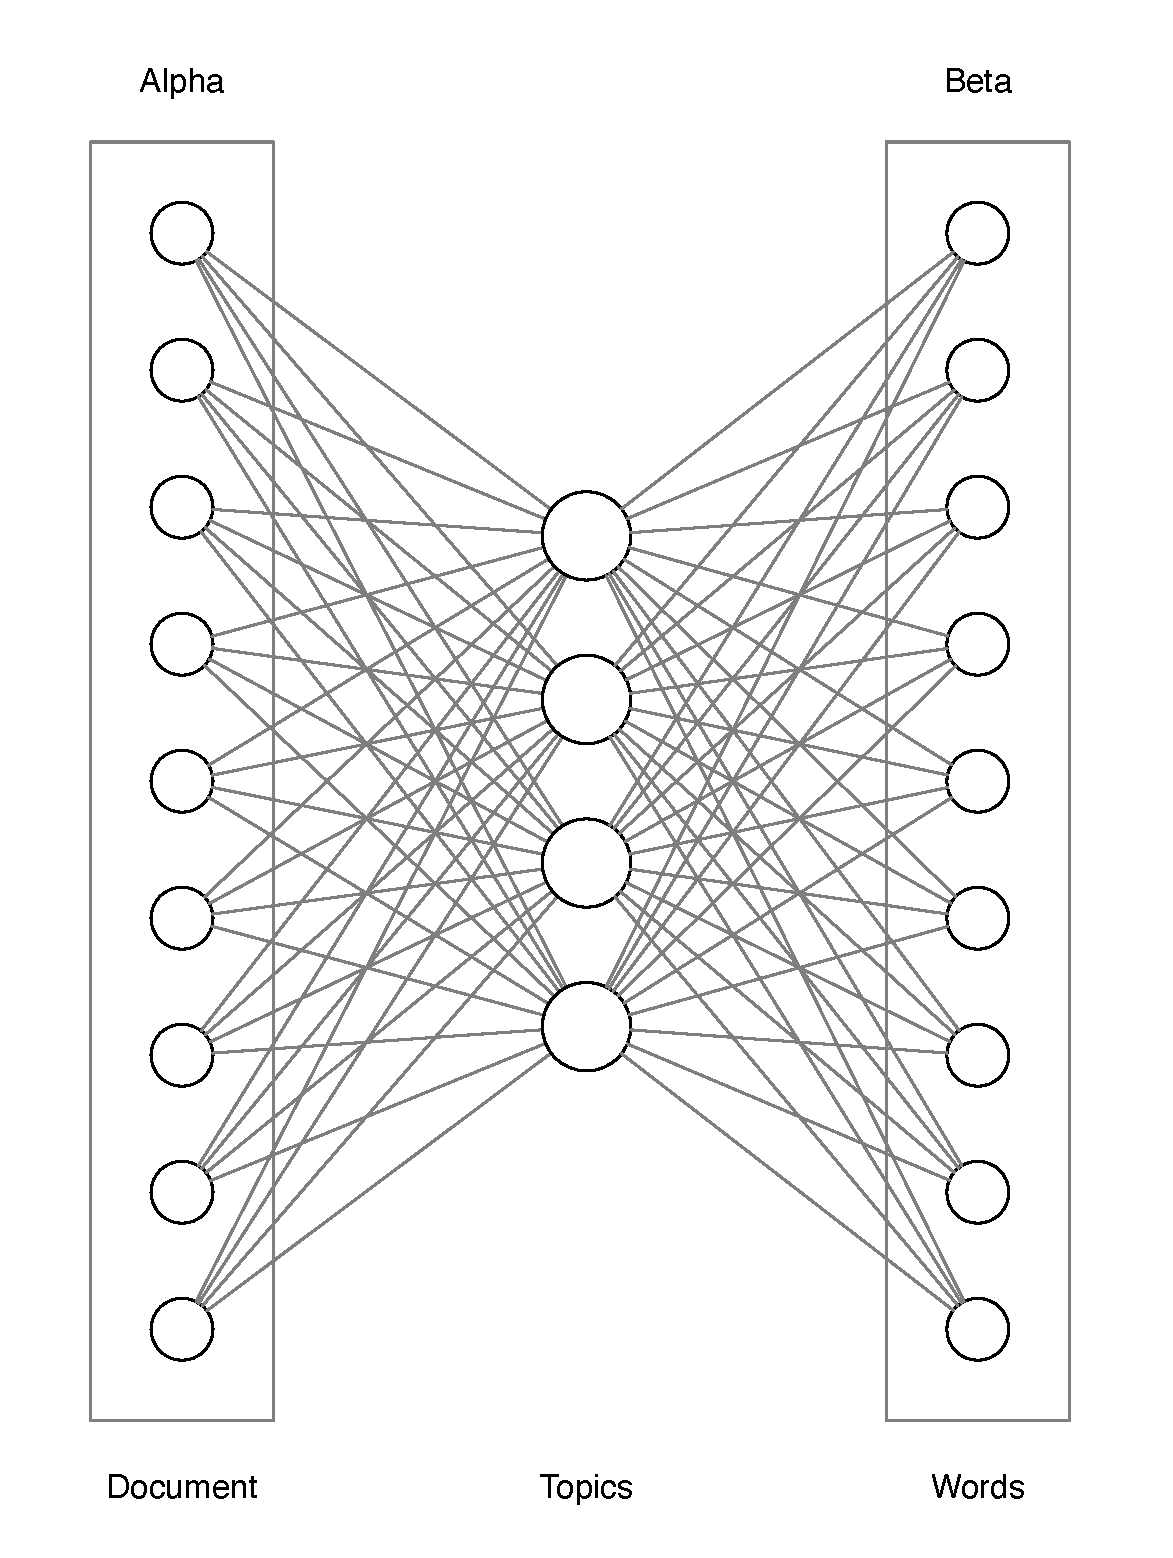
\includegraphics[width=12cm]{./figures/alpha1.eps}
\caption{Alpha and Beta representation}
\label{fig:alphaandbeta}
\end{figure}
In the rest of this section the lessons learned for both of these hyperparameters will be discussed.

\subsection{Dirichlet hyperparameter alpha}
Choosing a value of alpha and beta (eta) can be a tricky task, since these two hyperparameters has an direct impact on the topic modelling results. A high alpha means the documents contains more topics.

The researcher experimented with various alpha values. These values were 0.01, 0.1 and 0.5. It was discovered that using the above mentioned values, the actual prototype were displaying run time divide by zero errors. The cause of the errors were linked to the alpha and beta values. The model was producing explicit zero results.
As \citeA{wallach2009rethinking} mentions, an alpha asymmetric is good, but an asymmetric beta is not.
It was because of the run time errors, it was decided to set the parameters to auto. This means that the model learns an asymmetric statistical inference, or prior for short.

The hyperparameter beta will be discussed in the next sub section.
\subsection{Dirichlet hyperparameter beta}
It was also found that experimenting with various Beta (eta) values rendered the same run time errors observed with the alpha testing. The researcher has also decided to set the hyperparameter to auto, which learns asymmetric prior from the data.

This approach of setting the hyperparameters to auto, as stated prior, was found to benefit the topics generated by the LDA model. Giving the ability to the data to learn their own prior meant that it should deliver similar results each time the model ran. Capping or limiting the hyperparameters would result in run time errors and skewed results.

As mentioned by \citeA{griffiths2004finding}, when working with scientific documents, it is best to use a larger beta (eta) value. The reason is, it could lead to the model containing smaller number of topics and could cover more scientific concepts. In contrast to using a smaller beta (eta) value, which would produce more topics that would address specific concepts.

In the next section, similarities between the probability distributions will be discussed.
\section{Similarity between probability distributions}
In this section, lessons learned will be shared on the process of getting the similarity between the documents.

In section \ref{JSD}, Jensen-Shannon Divergence (JSD) was mentioned to be the improved method used to measure similarity between two probability distributions.
The researcher used the Jensen-Shannon Divergence method to calculate the distance between the two probability distributions. In recent years research has indicated that JSD still has relevance today \cite{tong2016text,giles2019subject,he2015topic,chu2010topic}.

As there are no parameters with Jensen-Shannon Divergence, it made it easy to implement it into the prototype and, ultimately look at the end results. Since the goal of this research was not to compare other similarity measurement methods, the researcher only considered JSD.

In the next section, the evaluating the output of the similarity of the probability distributions will be discussed.

\section{Evaluation} \label{ssec:eval}
In this section the observations between the test document and training documents will be discussed. Observations will be shared to understand if and what made the similarity list good or bad. 
In the next subsection a single test document with their corresponding list of similar documents will be discussed. The layout of the subsection will include observations on what made a topic like Digital forensics and it's similar documents good, what LDA parameters could contribute in the change of similar documents and how many documents matched. This structure will continue for what was considered a good match and a bad match.
\subsection{Digital Forensics}
The title of the test document was "Towards a Framework for Enhancing Potential Digital Evidence Presentation". The contents of the document covered workings towards a framework to develop methodologies and specifications. The ultimate goal is to effectively enhance the presentation and interpretation of any legal proceedings.

The recommendation list of documents of the above document consists of 5 documents. The list of recommendations are in table \ref{tab:digitalforensics}. Observing the list, one could argue that the topic, Digital Forensics, was a good topic to test with. 

\begin{table}[]
\centering
\resizebox{\textwidth}{!}{%
\begin{tabular}{|l|l|}
\hline
\textbf{JSD SCORE} & \textbf{TITLE} \\ \hline
0.5372 & TOWARDS A DIGITAL FORENSIC SCIENCE \\ \hline
0.6170 & A MODEL FOR SECURE VALUE-ADDED SERVICE SUBSCRIPTIONS IN CELLULAR NETWORKS \\ \hline
0.6172 & \begin{tabular}[c]{@{}l@{}}POPI ACT - OPT-IN AND OPT-OUT COMPLIANCE FROM A DATA \\ VALUE CHAIN PERSPECTIVE: A SOUTH AFRICAN INSURANCE INDUSTRY EXPERIMENT\end{tabular} \\ \hline
0.6179 & TEAM FORMATION IN DIGITAL FORENSICS \\ \hline
0.6306 & THE CURRENT STATE OF DIGITAL FORENSIC PRACTITIONERS IN SOUTH AFRICA \\ \hline
\end{tabular}%
}
\caption{Similarity for "Digital Forensic" topic}
\label{tab:digitalforensics}
\end{table}

The researcher has observed that one of the reasons why Digital Forensics was a good topic to test with was that there were multiple documents covering the same topic. This meant that the LDA model had more training data. Having multiple documents covering the same topic provided more words for the Bag-Of-Words representation of the text.

Another observation was that since Jensen-Shannon Divergence had no real parameters to adjust, little difference could be made in the greater scheme of things. Majority of the tweaking and working must be done before getting to the Jensen-Shannon Divergence. The tweaking was done in the text pre-processing, text representation and LDA model phases of the experiment.

\begin{lesson}[JSD no parameters]
Jensen-Shannon Divergence (JSD) does not have parameters to refine, thus putting more emphasis on the refinement of the pre-processing and topic modeling components.
\end{lesson}\label{L:JSD}

In terms of changing the LDA parameters, it was observed that when increasing the chunksize of the LDA model to cover all the documents in the training set yielded good results for this specific topic. In addition to that, increasing the number of passes during training also yielded good results.

In the next subsection, the topic Privacy, similarity list and observations will be discussed.
\subsection{Privacy}
The test document that was used had the title "Computer monitoring in the 21st century workplace" which layed out the foundation for a workplace privacy policy that protects the employee's.

The recommendation list has also provided the top 5 documents which it considers very similar to the document above. As viewed in table \ref{tab:digitalforensicsBA}, the titles of the documents does not indicate any privacy topics.

% Please add the following required packages to your document preamble:
% \usepackage{graphicx}
\begin{table}[]
\centering
\resizebox{\textwidth}{!}{%
\begin{tabular}{|l|l|}
\hline
\textbf{JSD SCORE} & \textbf{TITLE} \\ \hline
0.5612 & A PROFILE OF THE DISTANCE COMPUTING STUDENT SOFTLIFTER \\ \hline
0.5820 & CDMA IN SIGNAL ENCRYPTION AND INFORMATION SECURITY \\ \hline
0.6670 & CONTEXT AWARE MOBILE APPLICATION FOR MOBILE DEVICES \\ \hline
0.6671 & TOWARDS A FRAMEWORK FOR A NETWORK WARFARE CAPABILITY \\ \hline
0.6676 & ADAPTABLE EXPLOIT DETECTION THROUGH SCALABLE NETFLOW ANALYSIS \\ \hline
\end{tabular}%
}
\caption{Similarity for "Privacy" topic}
\label{tab:digitalforensicsBA}
\end{table}
The main observation for this subsection is that words that would be easier identifiable in the LDA model got lost in the pre-processing and LDA pipeline. 

The other observation was that once the number of topics increased, it created room for the other topics to also be included. Those topics were previously the second or third tier topics in the LDA model. 

\begin{lesson}[More is not better]
Increasing the number of topics increases the risk that topics will be included that does not provide any significant value.
\end{lesson}\label{L:more}

As simple as it may sound, compared to Digital Forensics, there was not a lot of documents which dealt with Privacy and workforce topics.

\section{Conclusion}

In this chapter, we discussed several themes while developing the prototype. What changes were needed to be made for the prototype to perform at its maximum. The other theme was the lessons that was learned while administering the changes. 

\begin{table}[]
\begin{tabularx}{\textwidth}{|l|X|}
\hline
\textbf{Lesson name} & \textbf{Lesson} \\ \hline
Goldilock's dilemma & The identification and removal of stopwords is a very important part of the pre-processing pipeline. Removing too much domain specific words does negatively influence the quality of the topics and, ultimately influence the similarity scores \\ \hline
Problematic ligature characters & Researchers using different tools for typesetting can make the pre-processing pipeline exclude words containing ligature characters \\ \hline
Manual intervention & When evaluating the quality of the topics generated by the model, even-though evaluation techniques like coherence scores or perplexity indicates good topics, manual intervention is still needed to validate them \\ \hline
Quality over quantity & Increasing the number of passes does not automatically increase the quality of the topics \\ \hline
Chunksize has little influence & Increasing the chunksize does not a significant influence on the quality of the topics \\ \hline
Probability Dilemma & If the minimum probability is set for too high, the topic model runs a risk to not include certain topics. Smaller documents often only have a few sentences which influences the probability of word occurring. Hence why the minimum probability can not be high \\ \hline
Flatten the curve & The perplexity score will flatten out as the number of topics gradually increase \\ \hline
JSD no parameters & Jensen-Shannon Divergence (JSD) does not have parameters to refine. Putting more emphasis on the refinement of the pre-processing and topic modeling components \\ \hline
More is not better & Increasing the number of topics increases the risk that topics will be included that does not provide any significant value \\ \hline
\end{tabularx}
\caption{Summary of the lessons learned}
\label{tab:lessons}
\end{table}

The lessons learned from each component, as indicated in Figure \ref{fig:prototype}, is summarised and shared in Table \ref{tab:lessons}. The conclusion that is drawn is that pre-processing is certainly one of the most important legs in the pipeline and needs to have most of the time dedicated to it. Each component of the pre-processing process needs to be closely considered. Removing too much words can cause documents not to any similarity to others and leaving too much words can make the LDA model too sensitive.

The experimentation, analysis and discussion enabled the creation of the model used in chapter \ref{chap: Chapter 6}. The model outline what steps were needed to achieve a recommendation list. It also opened discussions so researchers can further the research by using additional techniques and algorithms which will be discussed in the next chapter.